\chapter{Comparison of wind tunnel measurement and CFD simulation of a small plant}
\label{ch:wtcfdcomparison}
\def\figdir{chapters/ch06_wtcfdcomparison/figures}	

% description of the numerial method
% simulation domain description.
% boundary conditions
% how the leaf area density distribution is obtained
% comparison....

\lettrine[lines=3,nindent=0em,loversize=0.1]{I}{n} this chapter, we compare the numerical method described in \cref{ch:parametricstudy,ch:numericalmethod} with the measurements of \cref{ch:microclimatestudy}. The measurements were performed for a small \textit{Buxus} \textit{sempervirens} plant. The measurements consisted of: i) X-ray tomography measuring plant microstructure metrics such as net leaf area and leaf area density, ii) stereoscopic particle image velocimetry (SPIV) measuring the wake flow properties such as mean velocity and turbulence kinetic energy (TKE), iii) infrared thermography measuring the spatiotemporal leaf temperature profile, and iv) hygrothermal in-foliage measurement probes measuring the vertical distribution of relative humidity (RH) and air temperature. Therefore, the goal of the present study is to compare the numerical simulation of the Buxus plant setup using the porous medium approach detailed in this thesis and compare with the high-resolution dataset to quantify the discrepancies. The present study aims at providing insight to the feasibility of employing such numerical techniques and possible limitation.

\section{Simulation domain and boundary condition}

The simulation setup consisting of the numerical domain and its boundary conditions were that of the wind tunnel experiment with wind tunnel set wind speed $U_{\textit{ref}} = 1$ m\,s$^{-1}$. The reference velocity used for the study is the plant-canopy height velocity $U_H = 0.77$ m\,s$^{-1}$ at $H = 0.21$ m.

\subsection{Numerical domain}
	
	\begin{figure}[t]
		\centering
		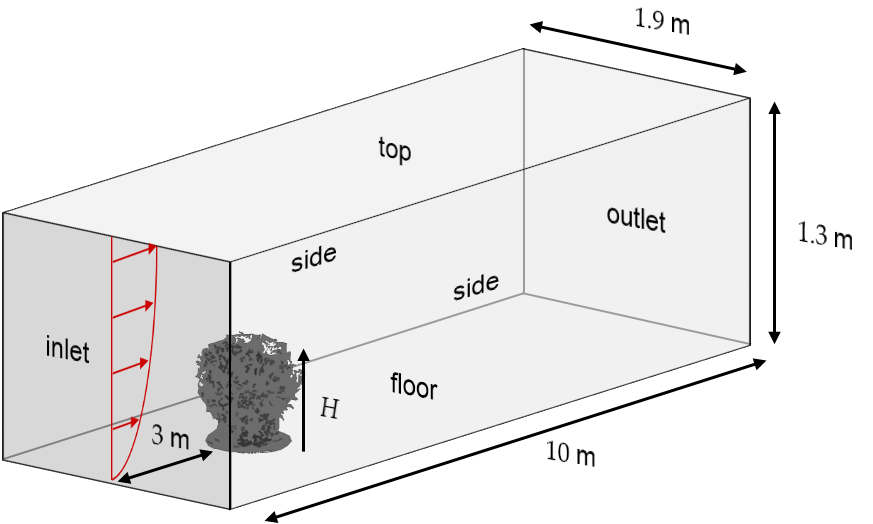
\includegraphics[width=0.8\textwidth]{\figdir/WT_CFD_comparison_setup_v2.png}
		\caption{Numerical domain used for the wind-tunnel-CFD comparison study with plant-canopy height $H = 0.21$ m (not to scale).}
		\label{fig:WT_CFD_comparison_setup}
	\end{figure}

The numerical domain is based on the geometry of the wind tunnel test-section with a wind tunnel height $H=1.3$ m and a lateral dimension $W=1.9$ m, as depicted in \cref{fig:WT_CFD_comparison_setup}. The downstream fetch of the numerical domain after the plant was extended to ensure a developed flow at the outlet of the numerical domain. %The plant frontal area is $A_{f} = 0.52$ m$^{2}$ and with a wind tunnel cross-sectional area of $A_{w}=3.04$ m$^2$, has a small blockage ration of $1.7$\%.

\subsection{Boundary conditions}

\begin{figure}[t]
	\centering
	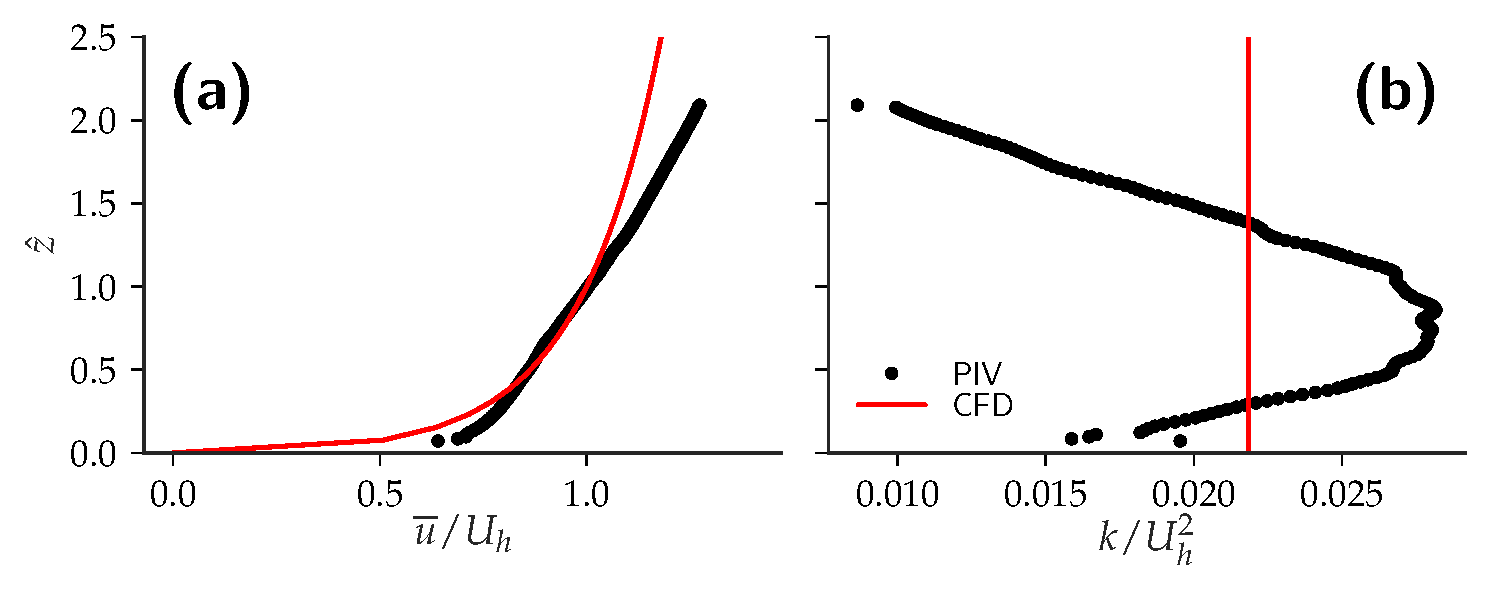
\includegraphics[width=0.8\textwidth]{\figdir/inletBoundarycondition_v2.pdf}
	\caption{Vertical profiles of incoming normalized \subfig{a} mean stream-wise velocity $\overline{u}/U_h$ and  \subfig{b} turbulent kinetic energy $k/U_h^2$ : (black) PIV profile from wind tunnel and (red) CFD boundary condition.}
	\label{fig:boundaryprofile}
\end{figure}

\cref{fig:boundaryprofile} shows the upstream boundary condition of mean velocity $\overline{u}$ (m\,s$^{-1}$) and the turbulent kinetic energy $k$ obtained from the wind tunnel experiment. An atmospheric boundary layer (ABL) profile, described through the following three equations \citep{Richards1993}:
\begin{align}
	\tavg{u}(z) &= \frac{{{u_*}}}{\kappa }{\text{ln}}\left( {\frac{{z + {z_0}}}{{{z_0}}}} \right) \\
	k &= \frac{{{u_*}^2}}{{\sqrt {{C_\mu }} }} \\
	\varepsilon  &= \frac{{u_*^3}}{{\kappa \left( {z + {z_0}} \right)}}
	\label{eq:ableq}
\end{align}
were used as the boundary condition at the inlet of the numerical domain, where $\tavg{u}(z)$ (m\,s$^{-1}$) is the mean horizontal velocity, $u_*= \num{0.062336}$ m\,s$^{-1}$ is  the friction velocity, $\kappa=0.41$ is von K\'arm\'an constant, $z_0 = \num{0.001335}$ m is the aerodynamic roughness height and $C_{\mu}=0.09$. The roughness height $z_0$ and the friction velocity $u_*$ were obtained using curve-fit of the measured PIV profile (see \cref{fig:boundaryprofile}), resulting in an inlet turbulent intensity of $I = \sqrt{2/3\,k}/U_{ref} = 12.1 \%$. The outlet boundary condition was defined as pressure outlet with a static pressure $p=0$. A zero-gradient boundary condition was enforced for $\mvec{u}$, $k$, and $\varepsilon$. The remaining boundaries (i.e., top-wall and side-walls) were modeled as no-slip wall-boundary and with standard wall functions.

\subsection{Leaf area density}

The vegetation is modeled as a porous medium parameterized using a leaf area density $a$ (m$^2$\,m$^{-3}$) distribution and a constant leaf drag coefficient $c_d$. The momentum source term $s_u$ (N\,m$^{-3}$) is given as:
	\begin{align}
		\mvec{s}_u &=  - \rho {c_d}a\left| \tavg{\mvec{u}} \right|\tavg{\mvec{u}} \\
			\label{eq:source_veg1}	
		s_k &= \rho {c_d}a\left( \beta _p \left| \tavg{\mvec{u}} \right|^3 - \beta _d\left| \tavg{\mvec{u}} \right|k \right) \\
		s_\varepsilon &= \rho {c_d}a\left( {{\beta _p}{C_{4\varepsilon }}{{\left| \tavg{\mvec{u}} \right|}^3}\frac{\varepsilon }{k} - {\beta _d}{C_{5\varepsilon }}\left| \tavg{\mvec{u}} \right|\varepsilon } \right)
		\label{eq:source_veg3}
	\end{align}
where $c_d$ is the leaf drag coefficient \citep{Wilson1977} and experimental measurements suggesting that $c_d \in \left[0.2, 0.5\right]$ \citep{Vogel1989}. The closure coefficients $C_{4\varepsilon}=0.9$ and $C_{5\varepsilon}=0.9$ are obtained from literature \citep{Katul2004, Kenjeres2013, Sanz2003}. The coefficients $\beta_p=1.0$ and $\beta_d=5.1$ are energy conversion ratio from MKE to TKE and TKE to heat, respectively. The valid parameters are dependent on the specific plant type and plant sample and require calibration. In this study, the X-ray tomography measured is used to determine the leaf area density $a$ distribution. Thereafter, the values are interpolated onto the numerical domain. In the present study, a simple tri-linear interpolation scheme is employed to interpolate onto the finite volume cells. The leaf area density $a$ is derived as: 
	\begin{equation}
	a = \frac{1}{2} A_l \frac{1 - \phi}{\int {1 - \phi }\,\mathrm{d}V}
	\label{eq:leafdensitywteq}
	\end{equation}
where $A_l$ (m$^{2}$) is the net plant leaf area (both sides of the leaves) and $\phi$ is the plant porosity. 

\subsection{Numerical solution}

The problem is solved using the SIMPLE pressure-velocity coupling algorithm, obtaining a steady-state solution. The gradient terms are discretized using Gauss integration and interpolated using second-order central differencing scheme (\texttt{linear}). Similarly, the divergence terms are interpolated using second-order linear upwind differencing scheme (\texttt{linearUpwind}). The pressure is solved using geometric-algebraic multi-grid (GAMG) solver and preconditioned with diagonal incomplete-Cholesky (DIG) smoother, whereas velocity is solved using Preconditioned bi-conjugate gradient (PBiCG) solver with diagonal incomplete-LU (DILU) preconditioner. The matrix solvers are iteratively solved until the residuals of pressure are below $\num{1e-5}$ and below $\num{1e-6}$ for all the other variables. Furthermore, under-relaxation factors are used with $\alpha_p = 0.3$ for pressure, $\alpha_u = 0.7$ for velocity (ensuring $\alpha_p + \alpha_u = 1$) and $\alpha_k = \alpha_{\varepsilon}=0.5$. The under-relaxation factors are modified to $\alpha_p=0.7$ and $\alpha_u=0.3$ for the non-isothermal case to ensure stable convergence.

\section{Isothermal case}

The comparison of the CFD simulation and the wind tunnel results are split into two section: \textit{isothermal} case and \textit{non-isothermal} case. In the isothermal case, the influence of the leaf area density distribution, plant drag coefficient, and the turbulence model is investigated. A preliminary assessment of the discrepancy between CFD and wind tunnel results is performed by comparing the mean velocity and TKE of the plant wake. Thereafter, the non-isothermal case investigates the vertical profile of the air temperature and relative humidity for both the daytime and nighttime conditions.

\begin{figure}[t]
	\centering
	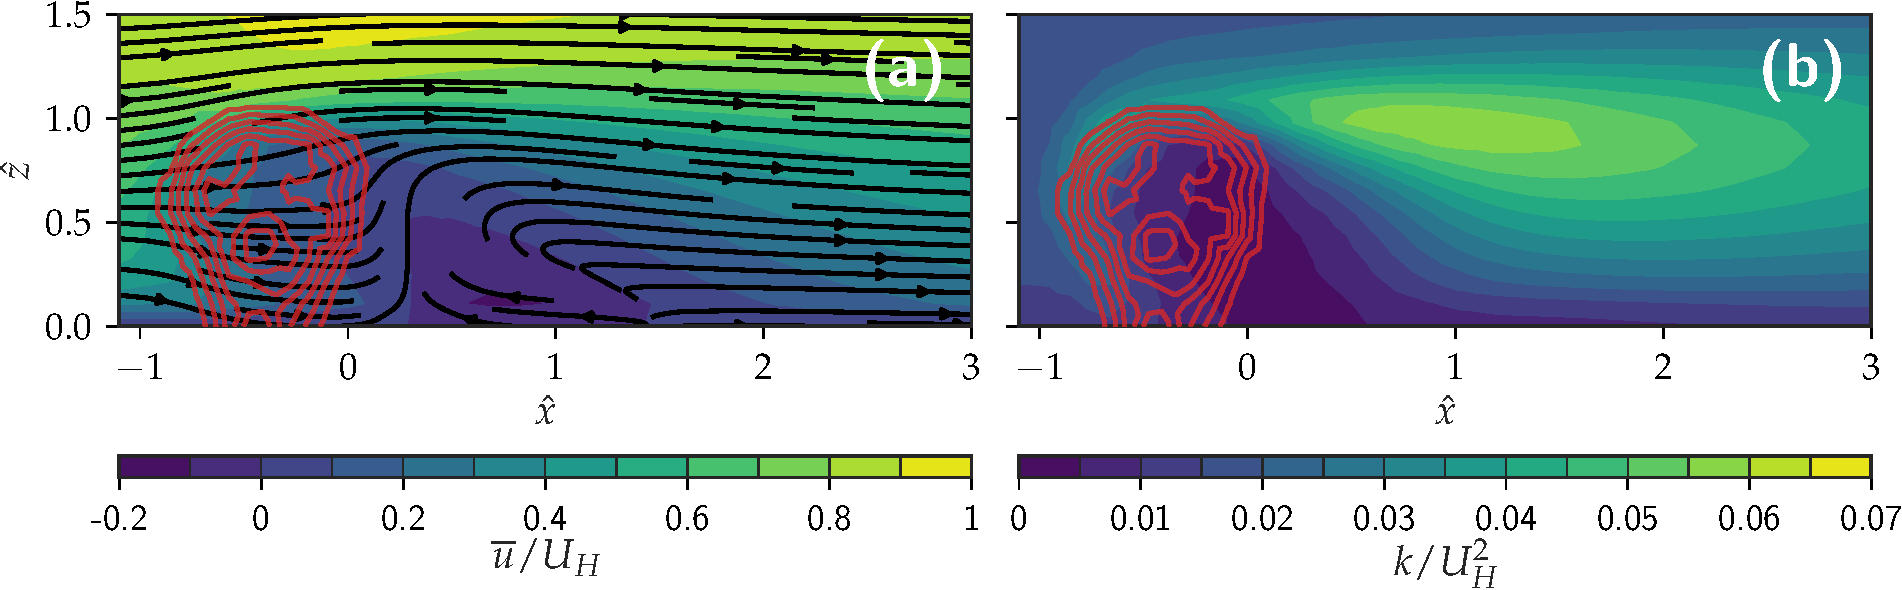
\includegraphics[width=\textwidth]{\figdir/basecase_vertical_UTKEstreamline-crop.pdf}
	\caption{Vertical plane at the center-line (i.e., at $\hat{y}=0$) showing the normalized \subfig{a} streamwise velocity $|\overline{u}|/U_H$ and \subfig{b} turbulent kinetic energy $k/U_H^2$ around the plant. The heterogeneous leaf area density $a$ is indicated with red iso-contour lines of $a = [20$, $40$, $60$, $80$, $100$, $120$, $140]$ m$^2$\,m$^{-3}$. The drag coefficient is $c_d=0.5$. Note that the corrected reference velocity $U_H = 0.95$ m\,s$^{-1}$ is used \citep{Blocken2007b}.}
	\label{fig:basecase_vertical_UTKEstreamline}
\end{figure}

\cref{fig:basecase_vertical_UTKEstreamline} shows the stream-wise velocity $|\overline{u}|/U_H$ and TKE $k/U_H^2$ due to the plant. The leaf area density is depicted using the iso-contour lines of $a = [20$, $40$, $60$, $80$, $100$, $120$, $140]$ m$^2$\,m$^{-3}$ determined using \cref{eq:leafdensitywteq}. It is seen to vary in space with peak density located approximately in the middle of the plant ($\hat{x}=-0.5$, $\hat{z}=0.5$). A modification to the reference velocity for the numerical model is seen to be necessary due to the bias in the CFD prediction. The airflow and TKE is seen to be consistently over-predicted. However, with a corrected reference velocity of $U_H = 0.95$ m\,s$^{-1}$ the flow field is seen to be in better agreement. The source of the bias is assumed to be the ABL inlet boundary condition. An apparent amplification of the velocity and TKE is observed in the CFD results, and similar finding has been observed by \cite{Blocken2007b}. However, a rigorous study of the source of the bias has not performed for this study. The vertical plane velocity field is plotted together with the streamlines (\cref{fig:basecase_vertical_UTKEstreamline}a). The near-wake of the plant is consists of a recirculation zone below $\hat{z} = 0.5$, indicated by negative stream-wise velocity. The highest TKE is observed at the plant-canopy height $\hat{z} = 1$, with peak TKE at approximately $\hat{x} = 1$. Therefore, the wake turbulence is seen to dominantly affected by the shear-zone generated by the plant canopy.

A preliminary comparison of the numerical prediction and the experimental measurement is performed by comparing the stream-wise velocity and the TKE at $\hat{x} = [0.4$, $0.6$, $0.8$, $1.0$, $1.2$, $1.4$, $1.6]$. \cref{fig:basecase_horizprofile_UTKE} shows the vertical profiles at these seven locations, where the lateral position is at the plant center-line (i.e., $\hat{y} = 0$).  The comparison shows a reasonably accurate prediction of the near-wake statistics of the plant. The prediction especially demonstrates an accurate prediction of the magnitude and the gradient of the stream-wise velocity. Although, very close to the tree, $\hat{x} < 0.6$, the deficit in the velocity is seen to be under-predicted. The TKE shows a good comparison as well with an accurate prediction of the peak TKE at the plant-canopy shear-layer. However, as with the stream-wise velocity, very close to the tree, there is a slight overestimation. Furthermore, the variability in height is seen to less severe than the experimental observation. This is most likely due to the numerical approach being a porous media approach where instead of explicitly resolving the plant elements (i.e., branches and leaves), they are aggregated into a distribution function.

\begin{figure}[t]
	\centering
	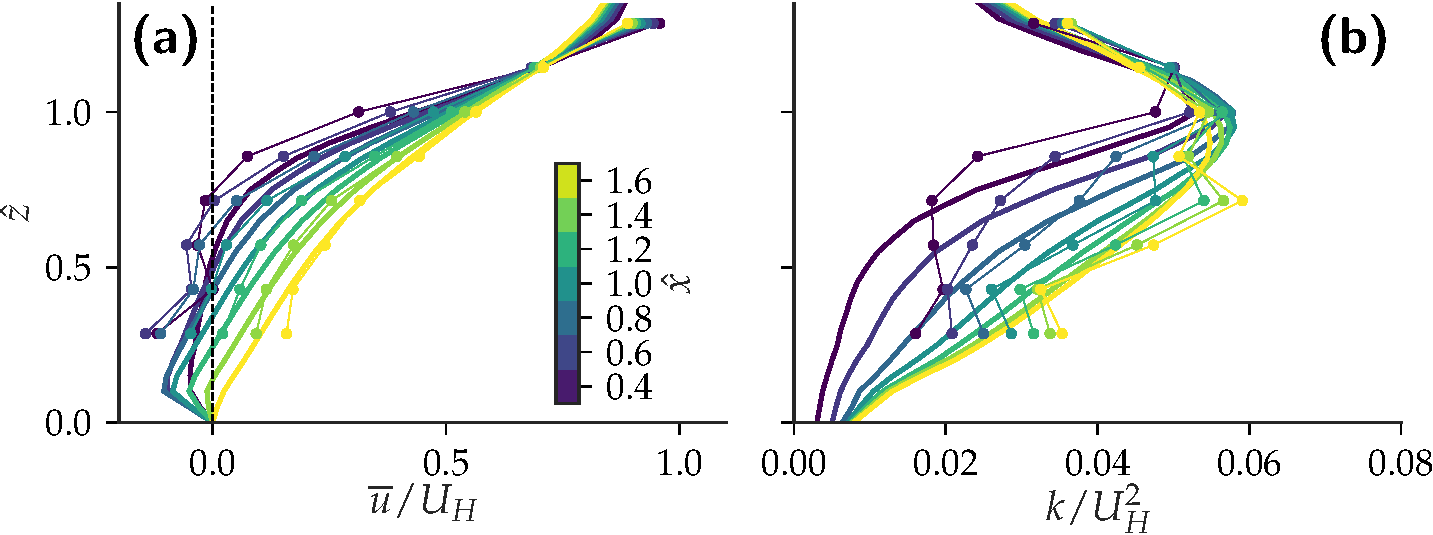
\includegraphics[width=\textwidth]{\figdir/basecase_horizprofile_UTKE-crop.pdf}
	\caption{Mean normalized vertical profiles at 7 streamwise positions $\hat{x}$, at center-line of the plant $\hat{y} = 0$: \subfig{a} streamwise velocity $|\overline{u}|/U_H$ and \subfig{b} turbulent kinetic energy $k/U_H^2$. Note that $U_H^{\mathit{exp}} = 0.77$ m\,s$^{-1}$ and $U_H^{\mathit{num}} = 0.77$ m\,s$^{-1}$. }
	\label{fig:basecase_horizprofile_UTKE}
\end{figure}

\subsection{Influence of heterogeneity in leaf area density distribution}

The influence of heterogeneity in the leaf area density distribution is investigated by comparing a spatially \textit{varying} leaf area density and a spatially \textit{constant} (average) leaf area density. Applying a spatial averaging operator to \cref{eq:leafdensitywteq}, we obtain the average leaf area density $\langle a\rangle$  (m$^2$\,m$^{-3}$) as:
	\begin{equation}
	\langle a \rangle = \frac{1}{2} {A}_l \frac{1 - \langle \phi \rangle}{\int {1 - \phi }\,\mathrm{d}V}
	\label{eq:leafdensitywteqaverage}
	\end{equation} 
where it is simply related to net leaf area $A_l$ and the average plant porosity $\langle \phi \rangle$. Therefore, the constant leaf area density distribution function in the air domain $\Omega_a$ is defined:
\begin{equation}
a(\mvec{x}) =
	\begin{cases}
	\langle a \rangle       	  & \quad \text{if}\ 0\le \phi < 1\\
	0  							  & \quad \text{if}\ \phi = 1
	\end{cases}
	\label{eq:leafdensitywteqaveragefield}
\end{equation}

\cref{fig:LAD_constvsvarying} shows the two types of leaf area density distribution at $\hat{y} = 0$. A spatially-averaged leaf area density is seen to be around $\langle a \rangle \approx 80$ m$^{2}$\,m$^{-3}$, with maximum leaf area density $\max (a) = 140$ m$^{2}$\,m$^{-3}$. %Due to the interpolation of the leaf area density from the initial measurement dataset to the finite volume grid, the leaf area distribution is seen to have a blurring effect at the edges. 

% However, due to the mesh discretization, the leaf area density distribution of \textit{constant} is seen to ``diffused'' (or ``blurred'') at the interface of the plant region. With increased mesh resolution, this edge-effect can be overcome.
	
\begin{figure}[t]
	\centering
	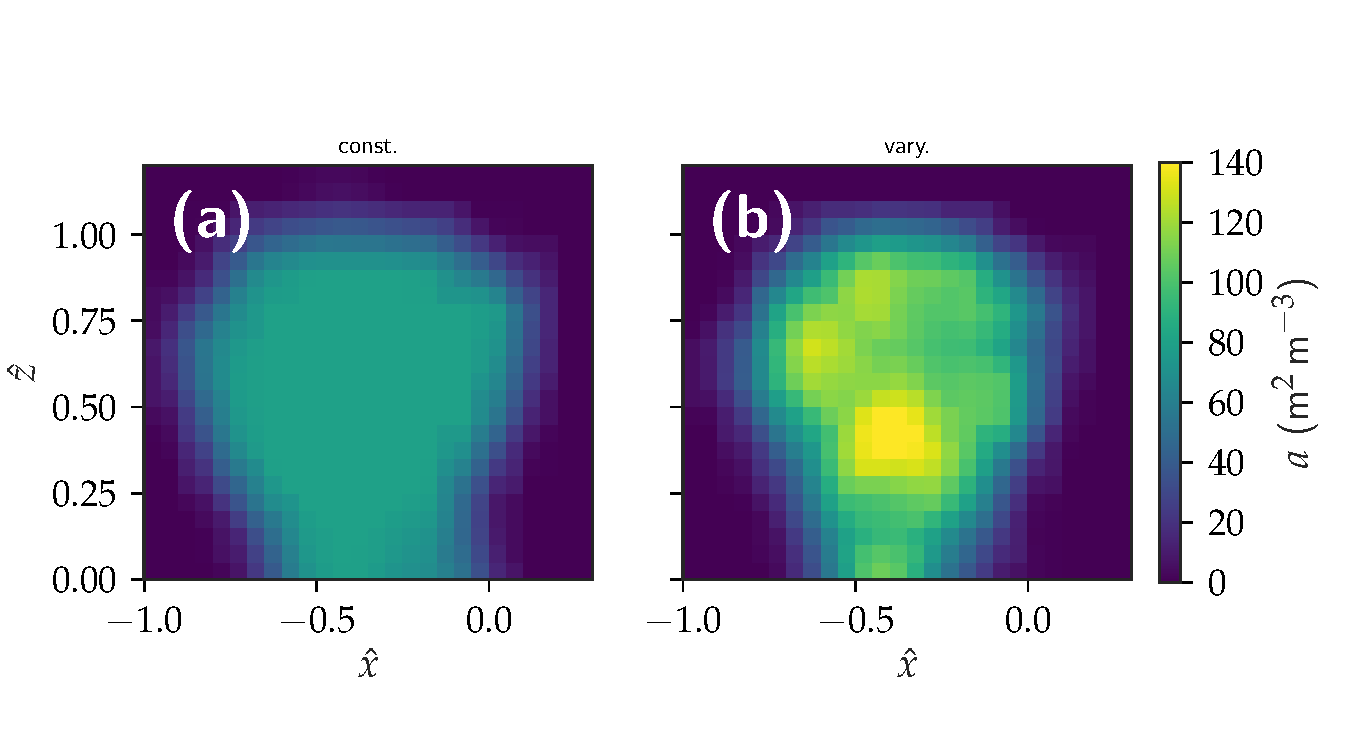
\includegraphics[width=\textwidth]{\figdir/LAD_constvsvarying_v2.pdf}
	\caption{Two types of leaf area density $a$ distribution: \subfig{a}  constant distribution and \subfig{b} varying distribution.}
	\label{fig:LAD_constvsvarying}
\end{figure}

\begin{figure}[p]
	\centering
	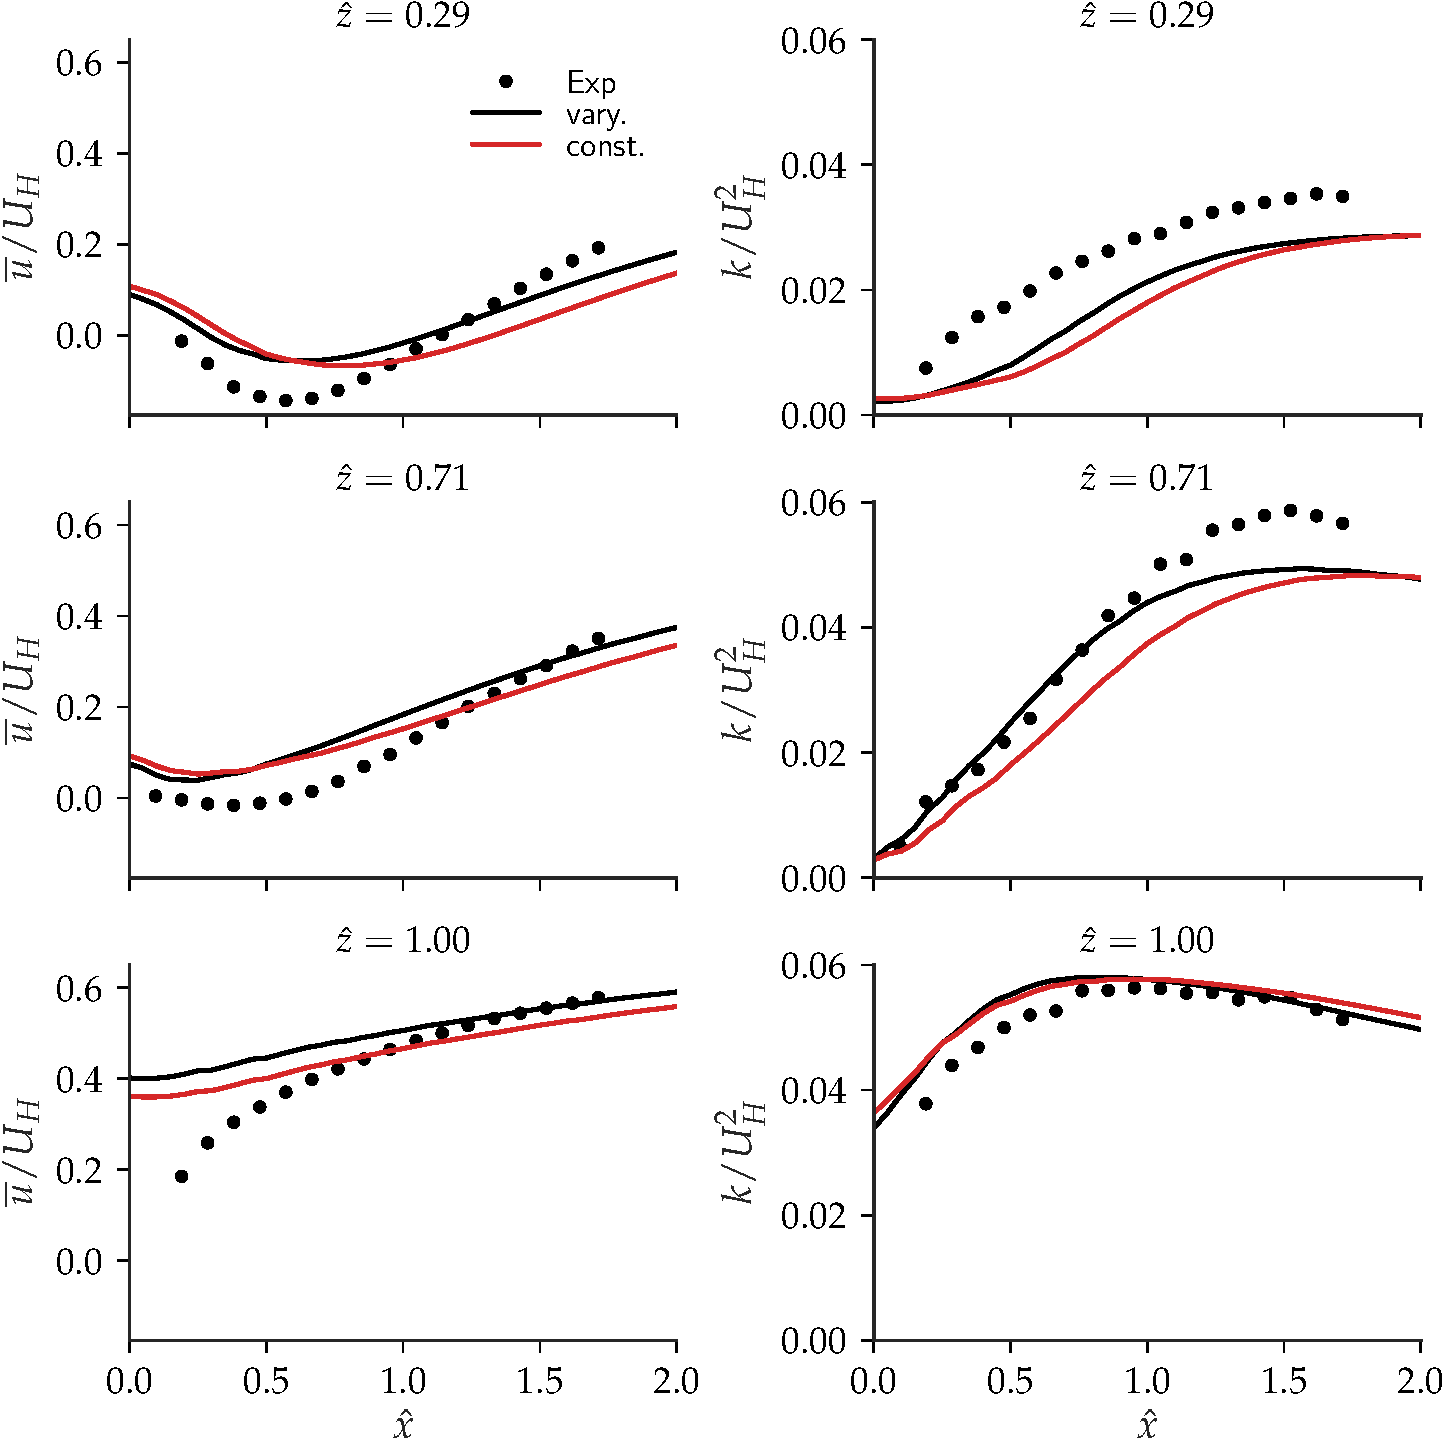
\includegraphics[width=\textwidth]{\figdir/WTvsCFD_LAD-crop.pdf}
	\caption{Influence of constant and varying leaf area density $a$ (m$^2$\,m$^{-3}$): Horizontal profile of normalized stream-wise velocity $\overline{u}/U_H$ and turbulent kinetic energy $k/U_H^2$ at heights $\hat{z} = [0.29$, $0.71$, $1]$.}
	\label{fig:WTvsCFD_LAD}
\end{figure}

To study the impact of heterogeneity in leaf area density distribution, both cases are compared with the wind tunnel measurements. \cref{fig:WTvsCFD_LAD} shows the horizontal profile of  stream-wise velocity and turbulent kinetic energy at three heights $\hat{z} = [0.29$, $0.71$ $1]$.  The figure reveals that both constant and varying leaf area density distribution shows similar behavior where the more realistic description of the varying leaf area density distribution is seen to provide better predictions. The stream-wise velocity profile shows that the numerical model under-predicts the peak wake velocity deficit at all heights. Furthermore, the wake recovery from the numerical model is seen to be slower than the measurements. Therefore, the recirculation length of the numerical model is seen to be larger than in reality. One of the possible contributing factors to the recirculation length is the accuracy of the turbulence closure. Therefore, the influence of the turbulence model is investigated in more detail. 

\subsection{Influence of plant drag coefficient}

A second plant property that determines the net influence of the vegetation on the flow is the drag coefficient $c_d$ in \crefrange{eq:source_veg1}{eq:source_veg3}. Generally, the drag coefficient is associated with the leaf drag coefficient and determined to be  $c_d \in [0.2, 0.5]$ \citep{Vogel1989,Wilson1977}. However, as there is a high quantity of branch elements in the small Buxus plant, the validity of the assumption is investigated by a parametric study on the drag coefficient.

\begin{figure}[p]
	\centering
	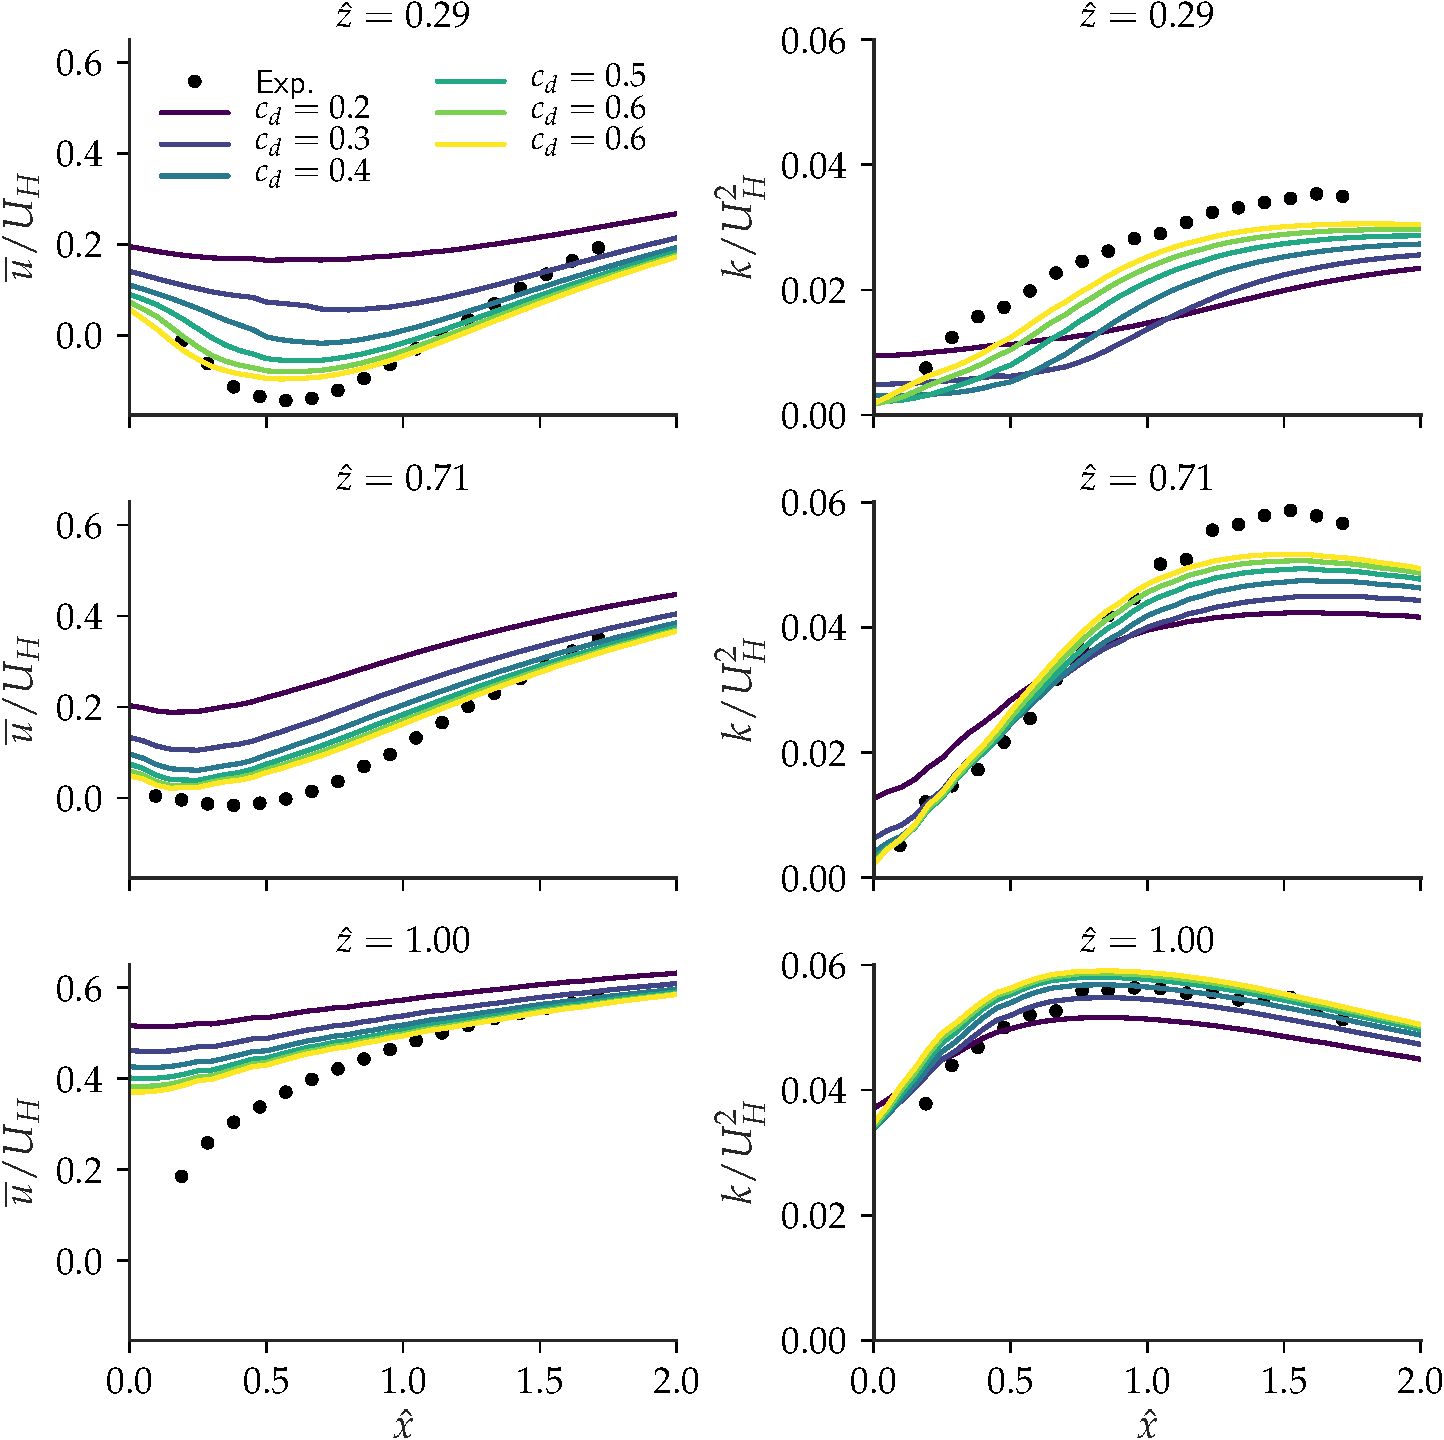
\includegraphics[width=\textwidth]{\figdir/WTvsCFD_cd-crop.pdf}
	\caption{Influence of drag coefficient $c_d = [0.2$, $0.3$, $0.4$, $0.5$, $0.6]$: Horizontal profile of normalized stream-wise velocity $\overline{u}/U_H$ and turbulent kinetic energy $k/U_H^2$ at heights $\hat{z} = [0.29$, $0.71$, $1]$.}
	\label{fig:WTvsCFD_cd}
\end{figure}

\cref{fig:WTvsCFD_cd} shows the horizontal profile of  stream-wise velocity and turbulent kinetic energy at three heights $\hat{z} = [0.29$, $0.71$, $1]$, and the influence of drag coefficient on them. We observe clearly that the numerical prediction convergently approaches to the experimental results as $c_d$ increases. Therefore, there is a clear indication that the drag coefficient of the plant is not just that of the leaf but should also take into account the contribution of the remaining plant elements such as branches. However, the wake velocity deficit still shows a slight under-prediction. Similarly, in the wake zone (i.e., $\hat{z} < 1$), the peak TKE is under-predicted. 


\subsection{Influence of turbulence model}

For the study of the turbulence model, four similar closure approaches were investigated: i) the standard $k-\varepsilon$ without vegetation terms, ii) the standard realizable $k-\varepsilon$ without vegetation terms, iii) the porous $k-\varepsilon$ with vegetation terms, and iv) the porous realizable $k-\varepsilon$ with vegetation terms.

\begin{figure}[p]
	\centering
	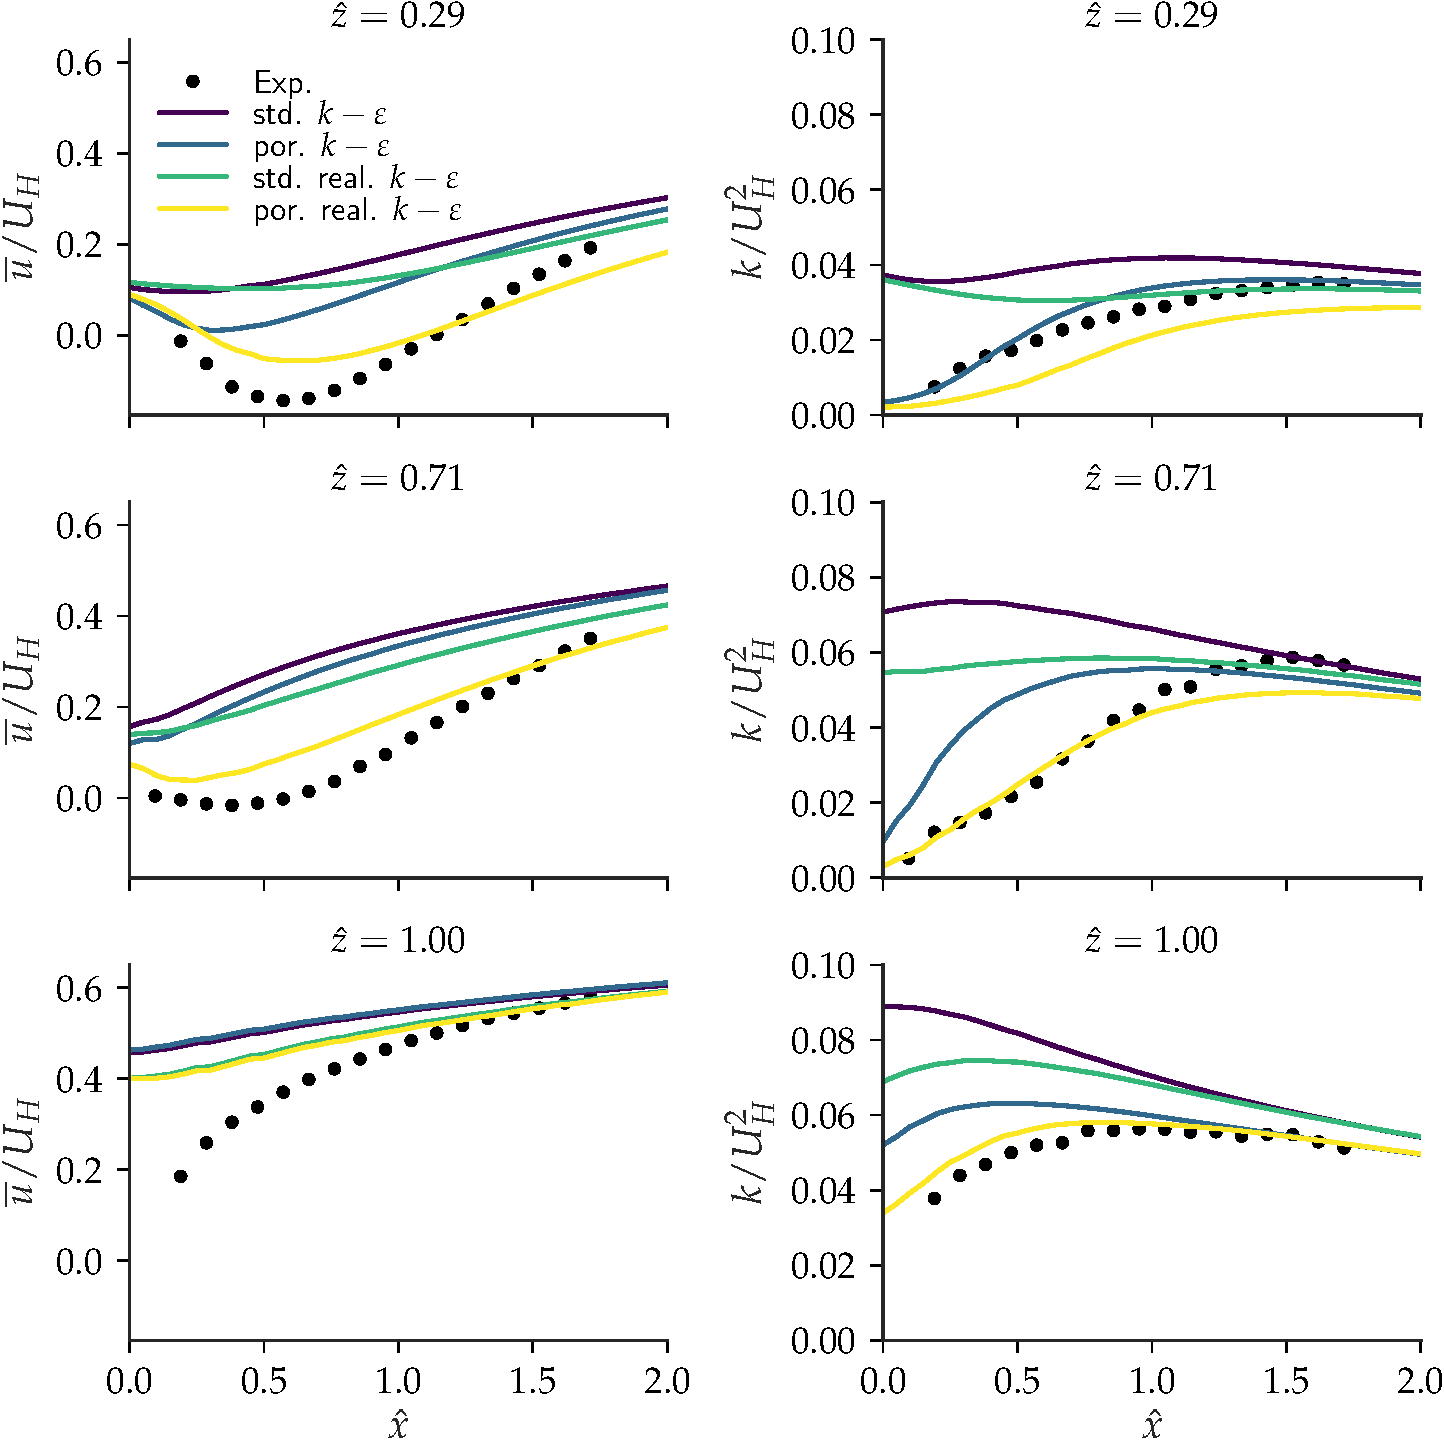
\includegraphics[width=\textwidth]{\figdir/WTvsCFD_RASModel-crop.pdf}
	\caption{Influence of turbulence model std. $k-\varepsilon$, std. real. $k-\varepsilon$, por. $k-\varepsilon$ and por. real. $k-\varepsilon$: Horizontal profile of normalized stream-wise velocity $\overline{u}/U_H$ and turbulent kinetic energy $k/U_H^2$ at heights $\hat{z} = [0.29$, $0.71$, $1]$.}
	\label{fig:WTvsCFD_RASModel}
\end{figure}

\cref{fig:WTvsCFD_RASModel} shows the influence the four turbulence closure approaches on the stream-wise horizontal profile of stream-wise velocity $u$ and turbulent kinetic energy $k$ at three heights $\hat{z} = [0.29$, $0.71$ $1]$. The study shows the clear importance of an accurate turbulence closure to obtain the real observed plant wake. Let us first look at the influence of the turbulence model by comparing standard $k-\varepsilon$ and realizable $k-\varepsilon$. We see that this change already has a good improvement to the numerical prediction. The realizable turbulence model is seen to outperform the normal $k-\varepsilon$ model providing more realistic velocity deficit and reduces the overestimation of the TKE. However, we see that the turbulence closure terms of the vegetation have a significantly stronger impact on the accuracy of the prediction. By adding the vegetation terms, i.e., the porous std. $k-\varepsilon$ is seen to be drastically better than the simple change of turbulence model from $k-\varepsilon$ to the more accurate realizable $k-\varepsilon$. We see that, not only is the wake velocity deficit more pronounced as with observation, but the TKE at the vicinity of the plant is seen to drastically less over-predicted. Therefore, the impact of foliage, such as the TKE suppression from the fluid-structure interaction of the foliage and airflow, is seen to be an important aspect of vegetation. As the standard turbulence models do not model such shortcuts in turbulence cascade (i.e., from TKE to heat), an over-prediction of turbulence is observed. The best performance in prediction accuracy is seen to be obtained from the porous realizable $k-\varepsilon$ model, where the stream-wise velocity deficit and the magnitude of the TKE is predicted with good accuracy. However, at the plant-canopy height (i.e., $\hat{z} = 1$), very close to the foliage (i.e., $\hat{x} \rightarrow 0$), the strong plant wake velocity deficit is not captured. This could be fundamentally due to the shortcomings of a porous media and similar immersed boundary approach where boundary layer flow phenomena are weakly captured. The flow characteristics prevalent the interfaces such as shear-flow are no longer captured with such spatial definition and intensity. 

An additional aspect of the turbulence closure is the model coefficients such as $c_{\mu}$, $C_{1\varepsilon}$, $C_{2\varepsilon}$, $C_{4\varepsilon}$, $C_{5\varepsilon}$, $\beta_p$ and $\beta_d$. These are also typically referred to as \textit{free} coefficients and typically requires rigorous calibration (i.e., tuned) to capture and recover the experimental observations. The calibration of these coefficient to the experiment results can be described as an optimization problem \citep{Margheri2014, Duraisamy2018, Couplet2005, Najm2009, Lucor2007, Gorle2015a, Gorle2013}, where data assimilation techniques are well regarded as an effective methodology to ensure the accurate, efficient convergence to global optima:
\begin{equation}
\mathop {\arg \min }\limits_{\mvec{c}}\ \epsilon(\mvec{x}, \mvec{c}) = \left\| {\mathcal{N}(\mvec{x}) - \mathcal{M}(\mvec{x},\mvec{c})} \right\|_2 
\end{equation}
where $\mvec{c}=({{c_\mu },{c_{1\varepsilon }},{c_{2\varepsilon }},{c_{4\varepsilon }},{c_{5\varepsilon }},{\beta _p},{\beta _d}})^T$ is a vector of the free coefficients and $\mvec{c}$ spans $\mathbb{R}^7$, $\mathcal{N}$ is the true Navier-Stokes solution (neglecting the experimental uncertainties) and $\mathcal{M}$ is the numerical model. Therefore, the numerical model can be regarded as a ``black-box'' simply dependent on the free coefficient vector $\mvec{c}$. We see that a brute-force search for coefficient vector $c$ that minimizes the error $\epsilon$ is intangible as the search needs to be formed in a 7-dimensional space, requiring a rigorous search algorithm. Therefore, the calibration of the turbulence model is beyond the scope of the study, but an important aspect for future studies. 

\section{Non-isothermal case}

\begin{figure}[t]
	\centering
	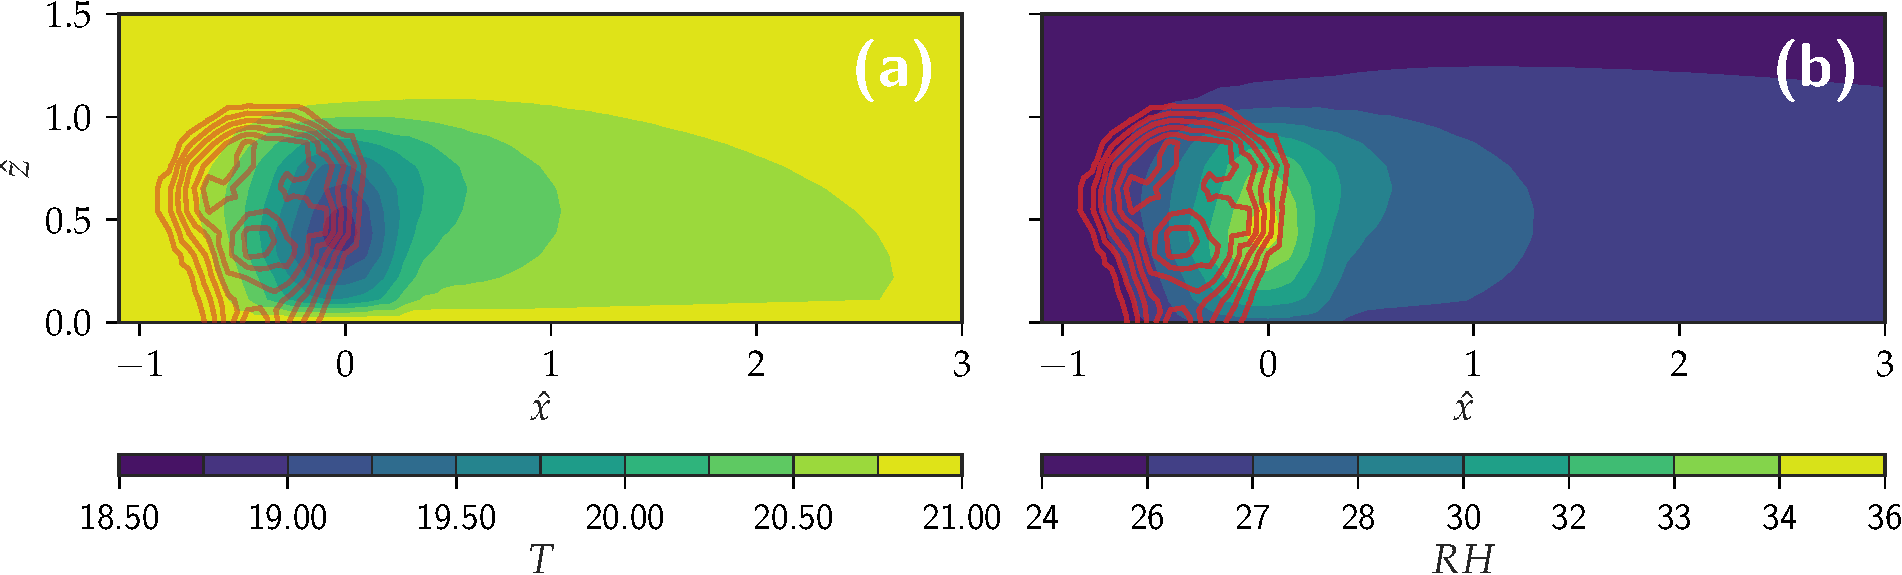
\includegraphics[width=\textwidth]{\figdir/vert_hygrothermal_plane-crop.pdf}
	\caption{Center-plane (i.e., $y=0$) hygrothermal condition of the flow at day-time with $T = 21$ $^{\circ}$C, $\textit{RH}=25$\% and $q_{\textit{r,sw,0}} = 100$ W\,m$^{-2}$: \subfig{a} air temperature $T$ ($^{\circ}$C) and \subfig{b} relative humidity $\mathit{RH}$ (\%).}
	\label{fig:vert_hygrothermal_plane}
\end{figure}

Finally, the numerical prediction of the thermal impact of the plant is compared with the hygrothermal wind tunnel measurements with ambient conditions $T = 21$ $^{\circ}$C, $25$\% relative humidity and plant-canopy incident solar radiation levels $q_{\textit{r,sw}} = \left[0,\ 100\right]$ W\,m$^{-2}$. The temperature and humidity equations are solved as passive scalar where the plant source is determined using the leaf energy balance approach described in \cref{ch:parametricstudy}. Additionally, the resistance-based aerodynamic and stomatal models described in the chapter are used to parameterize the heat and mass flux between the foliage and air. The minimum stomatal resistance of the plant is set to $r_{\textit{s,min}} = 400$ s\,m$^{-1}$, a typical value for deciduous plants \citep{Baille1994,Bruse1998}. Furthermore, it is equivalent to a stomatal conductance of $k_{\textit{st}} = 40$ mmol\,m$^{-2}$\,s$^{-1}$, typical of a \textit{Buxus} \textit{sempervirens} \citep{Rodriguez-Calcerrada2013a,Letts2012}. In our study, the characteristic plant leaf size is set to $l=3$ cm, obtained from measurements.

\cref{fig:vert_hygrothermal_plane} shows the temperature and relative humidity at the center-plane of the plant ($y=0$) during day time. A peak temperature drop of approximately $\Delta T = -2.5$ $^{\circ}$C and humidity rise to $\Delta RH = +12$\% is observed near the mid-aft region of the plant ($\hat{x} = 0$, $\hat{z} = 0.5$). We also note that there is no observed heating of the flow, typically present at the plant canopy height, possibly due to the lower level of incident solar radiation $q_{\textit{r,sw,0}} = 100$ W\,m$^{-2}$ and high convective heat transfer arising from the presence of wind. To accurately assess the discrepancy between the hygrothermal prediction and the experiment observation, the in-foliage air temperature, and relative humidity are compared at various vertical locations. \cref{fig:figure_airtemperature_relativehumidity_profile2} shows the vertical profile of the air temperature and relativity humidity during day and night where the results of the numerical simulation are plotted with dashed lines. In general, we see a good agreement with the numerical predictions and the experimental measurements. Although, we see that there is a slight overestimation of the transpirative cooling indicated by slightly lower air temperature and a slightly higher relative humidity during the daytime. The air temperature is seen to have the highest discrepancy at the top region of the foliage, where the solar radiation is intercepted. The air temperature is seen to be higher than ambient from the experimental observations. However, in the simulation, the air temperature is only seen to be lower than ambient indicating that a heat of the air, due to excess radiation absorption, is not numerically predicted. The numerical model predicts a transpiration rate high enough to reduce the air temperature. Comparing the relative humidity profiles, we see that the peak humidity from simulations is seen in the middle region of the plant (i.e., $\hat{z}=0.5$). At night, the hygrothermal parameters are well predicted with a minimal discrepancy. 

\begin{figure}[t]
	\centering
	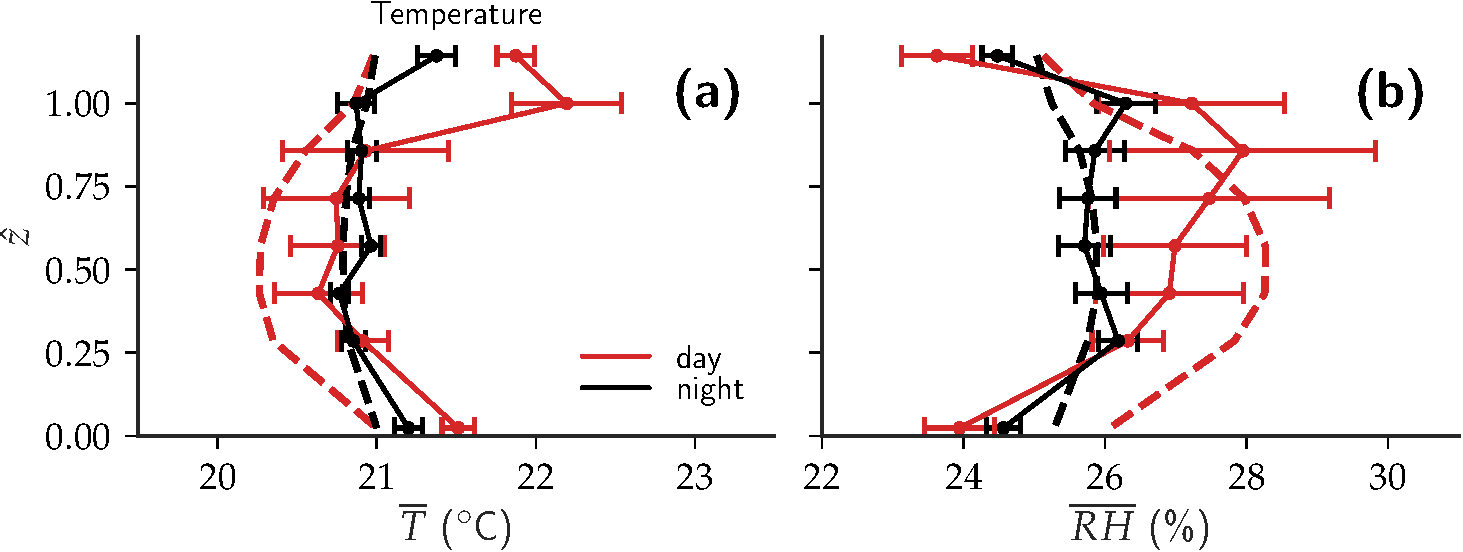
\includegraphics[width=\textwidth]{\figdir/figure_airtemperature_relativehumidity_profile-crop.pdf}
	\caption{Comparison of wind tunnel (solid) and numerical simulation (dashed): \subfig{a} Air temperature $T$ ($^{\circ}$C) and \subfig{b} relative humidity $\mathit{RH}$ (\%)}
	\label{fig:figure_airtemperature_relativehumidity_profile2}
\end{figure}

A more general assessment on the prediction of the plant transpiration can be assessed by examining the net plant transpiration rate during day and night. \cref{tab:nettranspirationcomp} shows the experimental and numerical value of the net transpiration rate $\textit{TR}$ (g\,h$^{-1}$) during day and night. The comparison validates the finding that numerical model predicts a high transpiration rate. Especially during the daytime, a very high transpiration rate of $17.6$ g\,h$^{-1}$ is predicted in contrast to the mean transpiration rate of $5.8$ g\,h$^{-1}$ and a peak transpiration rate of $14.8$ g\,h$^{-1}$. During the night, the net transpiration rate is predicted to be $4.9$ g\,h$^{-1}$, whereas the experimental observation suggests a mean and peak value of $3$ and $8.6$ g\,h$^{-1}$, respectively. Therefore, the numerical prediction of the plant transpiration is equivalent to the maximum plant transpiration rate. This indicates that time-dependent stomatal regulatory phenomena, as observed in chapter \ref{ch:microclimatestudy}, is not modeled using the presently used stomatal model. Furthermore, the comparison shows a need for a more rigorous modeling plant response to take into account dynamic plant responses.

\ctable[
	caption = {Experimental and numerical values of net plant transpiration rate $TR = \mathrm{d}m/\mathrm{d}t$ (g\,h$^{-1}$) during day and night.},
	label   = {tab:nettranspirationcomp},
	mincapwidth = \textwidth,
	pos = t,]{lrrr}{}{
\FL
	period		& \multicolumn{2}{c}{experimental}  	                        & numerical (g\,h$^{-1}$) \\
				&  mean  (g\,h$^{-1}$)	& max. (g\,h$^{-1}$)					&
	
\ML
	day 		&  $5.8$	            & $14.8$				                & $17.6$ \\
	night 		&  $3.0$                & $8.6$					                & $4.9$
\LL}

\section{Conclusion}

In conclusion, the numerical model is compared with the experimental measurements of a \textit{Buxus} \textit{sempervirens} plant. The non-isothermal comparison study focused on the prediction accuracy of the mean airflow and the turbulence modification due to vegetation. The non-isothermal study concluded that spatially resolved formulation of the leaf area density provides a more accurate description of the velocity deficit and the turbulence kinetic energy of the wake. However, the drag coefficient of the plant was seen to play a major role in the wake velocity statistics. With increasing drag coefficient, the numerical prediction was seen to converge to the experimental measurements. Although, at the vicinity of the plant and plant canopy height of $z=H$, the wake velocity deficit is seen to be always underestimated. This is due to the shortcomings of a porous media approximation of the plant where typically, boundary layer flow phenomenon such as sharp velocity gradient is not able to be accurately captured as the geometry is not explicitly resolved. The non-isothermal comparison study was concluded with the assessment of the turbulence model. It was distinctly seen that the realizable $k-\varepsilon$ model with the vegetation source terms quantifiably outperforms other models. The vegetation source terms were seen to be crucial at accurately predicting the wake velocity deficit. Moreover, the additional terms needed to model the suppression of the turbulence kinetic energy of the wake due to the interaction of foliage and the airflow. In contrast, the standard models were seen to always over predict the TKE in the wake. Finally, the isothermal comparison study assessed the prediction accuracy of the hygrothermal flow parameters such as air temperature and the relative humidity, and the transpiration rate of the plant. It was observed that the numerical model over-estimated the transpiration rate of the plant and is more in line with the peak plant transpiration rate, both during day and night. The high transpiration rate resulted in a higher transpirative cooling as observed by lower air temperature and higher relative humidity inside the foliage. However, the discrepancy between the numerical model and the experimental measurements was seen be small with approximately $0.5$ $^{\circ}$C and $2\%$ difference in air temperature and relative humidity, respectively. Thus, the comparative study of the numerical model and the wind tunnel experiment measurements showed that the numerical model shows a satisfactory prediction of both the non-isothermal and isothermal flow parameters.